
\section{The Cumulus System}
\label{sec:architecture}


\subsection{Architecture}


\begin{figure}
\begin{center}
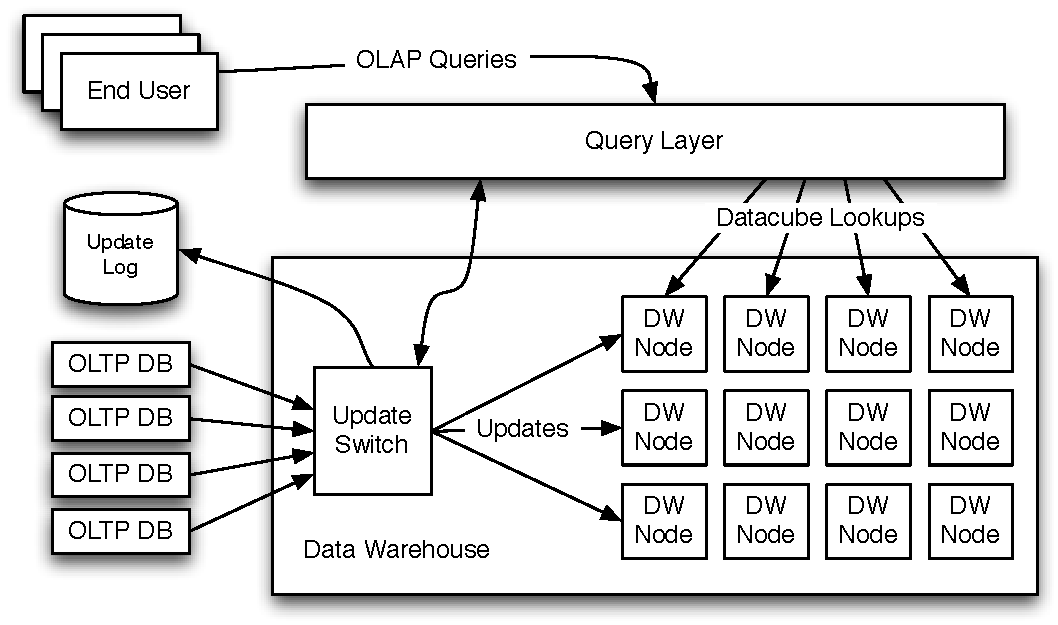
\includegraphics[width=3in]{images/Architecture.pdf}
\caption{Cumulus' architecture.}
\label{fig:arch}
\end{center}
\end{figure}


Cumulus consists of three components: the compiler,
a {\em runtime}, and a {\em query layer}.
A diagram of this architecture is presented in Figure \ref{fig:arch}.

The compiler, which was discussed in the
previous section, translates SQL aggregation queries
into message passing programs that are executed by the runtime system.

The runtime accepts updates -- insertions and deletes of tuples --
at a coordinator node called the \textit{Switch}, which delegates
update work to a number of data storage and query processing nodes, or
\textit{DW Nodes}.
The maps suggested by the compiler -- and maintained by the M3 program --
are partitioned across the DW nodes to keep network traffic to a minimum.  
The switch does not store any map data, but manages
the information about data placement (how maps are partitioned and which
partitions are located on which nodes).
Cumulus currently does only static data placement and does not migrate
data to balance load across DW nodes -- this is future work.

The runtime is designed to implement exact online aggregation, and
we conceive it to be used for main-memory OLAP.
The query layer accepts roll-up/drill-down/slice/dice queries,
instructs the Switch to have the DW nodes send a consistent version of
the relevant data to the querying node (the user's machine),
collects the result chunks there, and
finalizes the query answer
in a client-side API that runs on the user machine.

Our architecture supports the compilation of pre-aggrega\-tors close to the
OLTP database that reduce the load on Cumulus. For example, if sums of revenues
are to be computed, the revenues of batches of LineOrder tuples agreeing
on relevant join and group-by columns can be pre-aggregated close to the OLTP database and only this reduced workload of preaggregated tuples is sent to the Switch.

We generally assume that the data is persistent in the OLTP databases.
However, Cumulus is also able to
log the update stream arriving at the Switch and replay it from the
log later to recreate the data warehouse in main memory.
We could also log the map states using techniques as surveyed in
\cite{DBLP:journals/pvldb/SallesCSDGKW09}
for faster recovery, but this is currently not done.
We currently do not deal with node failures (which would naturally
be addressed using redundant data placement), and this is future work.


\subsection{Data Placement}


The Switch maintains information how map data is partitioned across
DW nodes. In the most general case, this would be a function
that maps a tuple update and a statement (id) from the M3 program to
a record that identifies, for each map access of the statement,
which DW nodes store any relevant data for executing this
statement.
%
In the curreny prototype of Cumulus, maps are partitioned along
dimensional axes, akin to the partitioning done in grid files\cite{318586}.


\begin{example}\em
\label{ex:switch_msg}
Consider the M3 program of Example~\ref{ex:ssb}.
Assume there are nodes $N_1$ to $N_5$,
which store the following map partitions:
\begin{eqnarray*}
N_1 &:& mPL[*, \mbox{odd years}] \\
N_2 &:& mPL[*, \mbox{even years}], mDL[*, \mbox{green parts}] \\ 
N_3 &:& mDL[*, \mbox{red parts}] \\ 
N_4 &:& m[*, \mbox{odd years}] \\
N_5 &:& m[*, \mbox{even years}]
\end{eqnarray*}

Suppose {\tt on insert into Date($d_1$, 2005)} is triggered.
The trigger consists of only one statement,
{\tt mPL[datekey, year] += 1}, where datekey and year are instantiated
with $d_1$ and 2005, respectively. Since 2005 is odd,
the map values to be written are located on node $N_1$.
The statement contains no map values to be {\em read}.

For {\tt on insert into LineOrder($d_1$, $p_1$, $500$)},
there is one statement, which reads from $mPL$ and $mDL$ and writes to $m$.
The tuple ($d_1$, $p_1$, $500$)
does not provide useful information for restricting the nodes to be contacted
in this case.
Values of $m$ may be located on $N_4$ and $N_5$, values of $mPL$ may be
located on $N_1$ and $N_2$, and values of $mDL$ may be located on $N_2$ and
$N_3$.
\punto
\end{example}


\subsection{Update Protocol}


\begin{figure}
\begin{center}
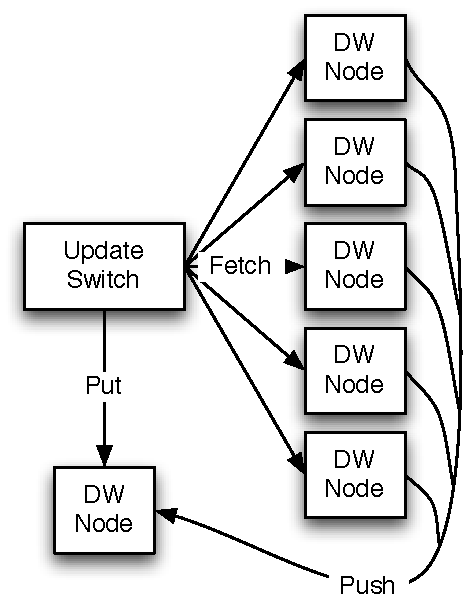
\includegraphics[width=1.5in]{images/UpdateStep.pdf}
\caption{Information flow during one map update.}
\label{fig:updatestep}
\end{center}
\end{figure}


On an {\em update} (an insertion or deletion of a tuple
$\vec{x}\vec{y}$), an M3 program processes a set of statements of the form
\[
\mbox{{\tt foreach $\vec{z}$ do} $m[\vec{x}\vec{z}]$ += $t$
~~~~~or~~~~~ $m[\vec{x}]$ += $t$}
\]
in {\em arbitrary}\/ order.
%
Each update has a sequence number (e.g., the $i$ if it is the $i$-th update
message received so far on the update stream. All messages sent by the
Switch contain this update sequence number.

For a given statement, the Switch proceeds as follows.
It composes a set of messages parametrized on $\vec{x}\vec{y}$ and
dispatches them to the DW nodes.
Nodes being read from are sent FETCH requests, which leads them to forward
PUSH messages containing the data read
to the appropriate writers. The writers are also
informed of their role by the Switch through PUT messages.

The update corresponding to an M3 statement is handled by the subset of
nodes that store partitions of the map being written to.  Each node
handles updates only for those partitions it stores locally. The Switch
uses the partition table to only contact readers who may store relevant information and writers who may have updates to do. 


As stated already, the nodes receiving a FETCH request perform the
requested reads and send their responses to the PUT nodes (the writers)
in a PUSH message.
The writers buffer received PUSH messages. For each write task to be
done, they receive a PUT message from the Switch which instructs them
what write to perform and which readers to expect PUSH messages from.
Readers who have received a FETCH message from the Switch always
send a PUSH message to the writers identified by the Switch in the FETCH
message: if a reader has no relevant data, it sends an empty PUSH message to
the writer to allow it to move on.
This allows the writer to know when all necessary PUSH messages have been
received and the write can be carried out.
An illustration of the complete message-passing process is given
in Figure \ref{fig:updatestep}.  


\begin{figure}
\begin{center}
\begin{tabular}{l|r@{~}l}
to node & & message \\
\hline
$N_1$ & FETCH($t$, & push mPL[$d_1$, *] to $\{N_4\}$) \\[.7ex]
$N_2$ & FETCH($t$, & push mPL[$d_1$, *] to $\{N_5\}$ and \\
      &            & push mDL[$p_1$, *] to $\{N_4, N_5\}$) \\[.7ex]
$N_3$ & FETCH($t$, & push mDL[$p_1$, *] to $\{N_4, N_5\}$) \\[.7ex]
$N_4$ & PUT($t$,   & {\tt foreach $(x,y)$ do} \\
      &            & ~~{\tt m[$x,y$] += 500 * mDL[$p_1$, $x$]} \\
      &            & ~~{\tt ~~~~~~~~~~~~~ * mPL[$d_1$, $y$]} \\
      &            & with messages from $\{N_1, N_2, N_3\})$ \\[.7ex]
$N_5$ & PUT($t$,   & {\tt foreach $(x,y)$ do} \\
      &            & ~~{\tt m[$x,y$] += 500 * mDL[$p_1$, $x$]} \\
      &            & ~~{\tt ~~~~~~~~~~~~~ * mPL[$d_1$, $y$]} \\
      &            & with messages from $\{N_1, N_2, N_3\})$
\end{tabular}
\end{center}

\vspace{-4mm}

\caption{Messages from the switch for Example~\ref{ex:switch_msg}.}
\label{fig:switch_msg}
\end{figure}



\begin{example}\em
\label{ex:switch_msg2}
We continue Example~\ref{ex:switch_msg} and take the partition choices
from there.
Suppose again that
{\tt on insert into LineOrder($d_1$, $p_1$, $500$)} is triggered and $t$ is
the sequence id of this update.
Then the switch sends the messages shown in Figure~\ref{fig:switch_msg}.
%
Let the current state of the maps be
mPL[$d_1$, 2005] = 1, mPL[$d_2$, 2006] = 1, mDL[$p_1$, red] = 1,
mDL[$p_2$, green] = 1. (These values are stored at nodes
$N_1$, $N_2$, $N_3$, and $N_2$, respectively).
Then the following PUSH messages will be sent:
\begin{center}
\begin{tabular}{ll|l}
from & to & message \\
\hline
$N_1$ & $N_4$ & PUSH($t$, mPL:$\{ [d_1, 2005] \mapsto 1 \}$) \\
$N_2$ & $N_4$ & PUSH($t$, mDL: $\emptyset$) \\
$N_2$ & $N_5$ & PUSH($t$, mPL:$\emptyset$; mDL: $\emptyset$) \\
$N_3$ & $N_4$ & PUSH($t$, mDL:$\{ [p_1, red] = 1 \}$) \\
$N_3$ & $N_5$ & PUSH($t$, mDL:$\{ [p_1, red] = 1 \}$) \\
\end{tabular}
\end{center}
\end{example}


In general, it is a goal of data placement
to partition maps in such a way that the number of
messages to be sent remains low. This can be done by collocating
corresponding partitions (via key-foreign key relationships)
of different maps on the same nodes.
In the previous example, the maps $m$ and $mDL$
could be partitioned on partkey and the partitions of $m$ and $mDL$ for the
same key ranges could be kept on the same nodes.
In the case of insertion of a LineOrder tuple, we would then know exactly
where to FETCH the mDL data; actually, this data would only have to be
PUSHed locally inside that node.


\subsection{Anatomy of a DW Node}


A DW Node receives and processes FETCH, PUSH, and PUT messages
as just described.
It has to process the messages it receives from the Switch 
in the order they are {\em sent}\/. For example, a
TCP connection with the Switch ensures this. Apart from protocol messages
that ensure in-order delivery of FETCH and PUT messages, the Switch receives no
messages from the DW Nodes.
The processing of received PUSH messages from other DW Nodes is done in the
order they are received, even though no particular order is
necessary for correctness.

Internally, each DW Node maintains committed versions (identified
by update sequence numbers) of the maps it maintains. In practice, we
will only need to keep a relatively small number of versions, and we will always know when an old version is not needed anymore and an be dropped.
Since consecutive versions only have small differences, we maintain
old versions as diffs to the latest version.

\begin{todo}
In addition, a DW Node has a buffer for received PUSH messages. 

An old version of map data has to be kept as long as there


Writing is done as follows:
The PUT nodes compute the update expression and modify the affected maps.  

Looping updates require the Switch to match corresponding read and write partitions.  The correspondence is obtained by identifying intersections between partitions of the target map that are affected by the update, and those of each map in the update expression.  This is equivalent to a join over components of the spatial index stored at the Switch.  Loop-free updates are a special case of this, where only one partition is required from each map.


{\em Get Collation}.
FETCH responses, or PUSH messages for an update are sent to the node managing the partition being updated.  Having received the number of FETCH messages sent by the switch with the PUT message, the destination node can buffer PUSH messages until all have arrived.  At this point, if the update is loop-free, the destination node simply uses the contents of the PUSH messages to evaluate the update expression.

If the update requires a loop, the destination node must do some processing.  The node first generates a set of tables, one for each map reference in the update expression.  Arriving map values populate tables that correspond to any map reference matching the value's keys, where loop variables act as wildcards.  When all values have been received, the destination node computes the natural join of all of the generated tables, effectively producing one update value for every assigned value in the domain of all of the loop variables.  The loop-free update is a special case of this where each generated table contains only one row.
\end{todo}


\begin{example}\em
\label{ex:switch_msg3}
We continue Example~\ref{ex:switch_msg2}.
Node $N_4$ knows from the PUT message that it will receive
one message with timestamp $t$ from $N_1$ with mPL values and one message each
from $N_2$ and $N_3$ with mDL values. It buffers those until it has receive
all three messages and then updates $m$ for all pairs of an mPL value and an
mDL value.
For

Node $N_5$ proceeds analogously.
\punto
\end{example}


\subsection{Message Ordering and Consistency}


In general, the order of execution among the statements of a single update
does not matter as long as all
statements read only map values not yet modified by other statements processing
this or a later update. This could be assured by a suitable topological sort of
the statements\footnote{Such a topological sort of the statements
assures that no map is read after it is written.
It is a property of our compilation approach that there are no cyclic dependencies between maps among the statements of a single update -- so a topological sort is always possible -- and the order in which the
compiler outputs triggers statements is already such a valid
topological sort.
We have implicitly performed such a topological sort in the M3 examples we have
shown so far and have shown trigger implementations as sequences of
statements.}, but in the Cumulus runtime we instead maintain versions of
the maps (and reads are always on the old version of the map).


The relative order by which the Switch sends messages
belonging to the execution of a single M3 statement does not matter.
However, messages from the switch to one and the same node
(those will have different timestamps) have to arrive there in order.
This can be made sure by using TCP connections between the switch and nodes
or simulating them.

Analogously, the order in which PUSH messages are sent or received does not matter.



\subsection{Old Consistency Stuff}


For consistency, an update's effect on the warehouse be logically atomic.  Atomicity is of particular importance, since the set of update rules triggered by a given update switch typically span the breadth of the data-dependency graph; Updates to any input relation typically have at least one read to a map updated by every other relation.

As the clearinghouse for updates, the Switch presents an ideal point for generating a total ordering over all tuples to be inserted into the warehouse.  The Switch maintains a version number for each node, incremented on every PUT dispatched to the node hosting it.  FETCHes sent to that node are tagged with the version number of the last PUT sent to the node, while PUTs are dependent on the completion of the prior PUT.

DW nodes ensure consistent evaluation of updates by buffering PUT requests received out of order, or prior to the completion of an earlier PUT request.  Similarly, FETCH requests for a particular version are buffered until the corresponding PUT request has completed, if it has not already done so.

Periodically, the switch queries each node for the completion status of pending PUT requests.  For each node, it computes the lowest FETCH version number for a read associated with an incomplete PUT request.  The Switch then disseminates these version numbers throughout the warehouse with a COMMIT message.  When a node receives a COMMIT, it snapshots its maps by discarding all updates for values that were overwritten before the commit version.




\nop{
\subsection{Precomputing message groups in the switch}

{\em Indexing message sets}.
To streamline the dispatch of messages to component nodes, the switch pre-generates a spatial index for each template\footnote{Elsewhere called map update statement. It is convenient to think of such a statement, particularly if it is of the {\tt foreach} form, as a template of message passing.}, similar to the grid file directory.  Every entry in the spatial index contains a set of PUT and FETCH messages.  When the template is triggered, the tuple's values are used to index into the spatial index and the corresponding messages are parametrized and sent.  The algorithm for generating the spatial index is presented in Figure \ref{alg:dispatch}.
} % end nop
